%================================================================================================% 
% thesis.tex                                                                                     %
% This is the main file, which calls up preamble.tex, front-matter.tex, and thesis.bib as needed. %
%================================================================================================%

% Front-matter shortcuts; note the extra space at the end, which is unfortunately necessary:      
\newcommand\myname{John P Gallagher }
\newcommand\mytitle{On a Topological Erdos Similarity Problem } % The graduate division requires this to be in caps.
\newcommand\mydegree{Master of Arts } % change to  Master of Science if applicable
\newcommand\myfield{Mathematics } % e.g., Mathematics
\newcommand\thismonth{May } % graduation month: May / August / December
\newcommand\thisyear{2022 } % e.g., 2014

\newcommand\myadviser{Dr. Chun-Kit Lai} % Adviser
\newcommand\myadviserstitle{Associate Professor}
\newcommand\committeememberone{Dr. Emily Clader} % Committee member 1
\newcommand\committeememberonetitle{Assistant Professor} 
\newcommand\committeemembertwo{Dr. Arek Goetz} % Committee member 2
\newcommand\committeemembertwotitle{Professor}

\documentclass[12pt,oneside]{sfsuthesis}  
%WHEN THESIS IS COMPLETED, CHANGE THE NEXT LINE FROM draft TO final, then the paper will be formatted according to the Graduate Division's guidelines
\usepackage[final]{MAThesisOutputFormat}
\RequirePackage{standalone}

%==========%
% biblatex %
%==========%

\usepackage[backend=biber,style=numeric]{biblatex}
\addbibresource{thesis.bib}

%=========================%
% CUSTOM PACKAGES GO HERE %
%=========================%

%\usepackage{TCbasic}

\begin{document}
\thesistitle

% Key words:\begin{itemize}
%     \item Dynamical Systems
%     \item Density and Measure are not clearly linked
%     \item Geometry
%     \item Fractals poorly defined
%     \item Self Similarity is more well defined
%     \item Cantor Set
%     \item $\R^n$ Fractals
%     \item Erd\"{o}s Proposed Conjecture with Measure Space assumptions
%     \item Theorem with Topological Assumptions.
%     \item Open questions
% \end{itemize}
% Main body of work:
\chapter{Introduction}

From the perspective of applied math, empirical results are almost always discrete observations yet the relationships that are observed are not necessarily quantized.  This means that as we infer mathematical relationships from discrete sets, there can often be a mismatch between our theoretical model, and the true relationships.  This notion of embedded relationships is also a core area of study within pure mathematics.  Whether observing a pattern and trying to generalize the relationship to a broader context, or deducing a relationship from a different set of assumptions, discrete patters are intrinsically embedded in our universe.  Indeed as we examine our world we often notice similarities we want to measure.  Using that same measure we want to look for consistency, and should we see something similar to our original observation we would expect a similar measure.  

However in mathematics (and life), the rules we construct often lack the subtly to account for nuances. Let us na\"{i}vely consider measurement.  Suppose we have a string and want to find out its length.  After pulling the string taught along a ruler, we might see it is a few centimeters long.  Then from this collection of tools we might say that we only need two points and a ruler to be able to describe length.  In reality we have only learned of distance.  

From that same construction though, we could just as well say, 2 points have no length at all because there is nothing between them.  In a sense, both are simultaneously true, because our definition does not address these nuances.  This motivates a few new questions: How many points do you need to add in, before we can have a length of string?  Can we use this string to measure other things?  Can we use collections of points to measure other things?  And maybe strangest of all, can collections of points have the same length as a piece of string?

We can now go back to our notion of the universe and ask ourselves these questions again.  Suppose we change universes, does our notion of length still exist? In a different universe can we find similar copies of these collections of points? 

Key words:\begin{itemize}
    \item Dynamical Systems
    \item Density and Measure are not clearly linked
    \item Geometry
    \item Fractals poorly defined
    \item Self Similarity is more well defined
    \item Cantor Set
    \item $\R^n$ Fractals
    \item Erd\"{o}s Proposed Conjecture with Measure Space assumptions
    \item Theorem with Topological Assumptions.
    \item Open questions
\end{itemize}

%\section{Introduction to the Introduction}



%\subsection{Introduction to the Introduction to the Introduction}



    %Patterns in Data sets
    %Def Affine Copy
    %Def Measure-Universal
    %State Erdos Conjecture
    %History/Context for Erdos Conjecture, 
        %Proposed Year
        %Who are main researchers?
        %What is current Progress?
    %Def Topological-Universal
    %Propose Analogous Theorem
    %Outline Paper Sections ahead
        %Measure ideas:
        %Topology ideas:
        %Gap Lemma
        %Main Thm
        %Multi-Dim Thm
\section{Affine Copies and the Self Similarity Property}

    %Patterns in Data sets
    %Def Affine Copy
    %Def Measure-Universal
    %State Erdos Conjecture
    %History/Context for Erdos Conjecture, 
        %Proposed Year
        %Who are main researchers?
        %What is current Progress?
    %Def Topological-Universal
    %Propose Analogous Theorem
    %Outline Paper Sections ahead
        %Measure ideas:
        %Topology ideas:
        %Gap Lemma
        %Main Thm
        %Multi-Dim Thm

One of the more popularly known results from math is the the Mandelbrot set fractal.  In some senses fractals can be very general objects that are considered to have fractional dimensions.  This definition can be very general but by that same token, may not always capture some of the inherent geometry of some fractal type objects. Some objects with fractional dimensions have a self-similar property, and some self-similar objects have fractional dimension.  For the scope of this paper, we will not be discussing dimension. However we will investigate the notion of self-similarity. 

We can now start by defining \textit{affine transformations} or \textit{affine copies}.
\begin{definition}[Affine copy]
    An \underline{affine copy} of a set $A$ is a scaled and translated set $A'$ such that for some $\lambda\neq 0, \lambda \in \R$ and $t \in \R$,  $$A' = \{\lambda a + t : a \in A\}.$$
\end{definition}

Even one dimensional objects can have this self-similar property. Take for example the middle Third Cantor set.  The middle third Cantor set is defined by recursively removing the open middle third interval of the previous remaining closed intervals.  Explicitly this can be constructed using countable intersection.  

\begin{example}[The Middle Third Cantor Set]\label{middleThirdCantor}
    $$\mathcal{C} = [0,1] \setminus \bigcup_{n=0}^\infty\bigcup_{k=0}^{3^n-1}\left(\frac{3k+1}{3^{n+1}},\frac{3k+2}{3^{n+1}}\right)$$
\end{example}

This set in particular exhibits this self-similar property because each level is a scaled copy of the entire object.  The following figure shows the first seven intervals removed.  

\begin{figure}[h]
    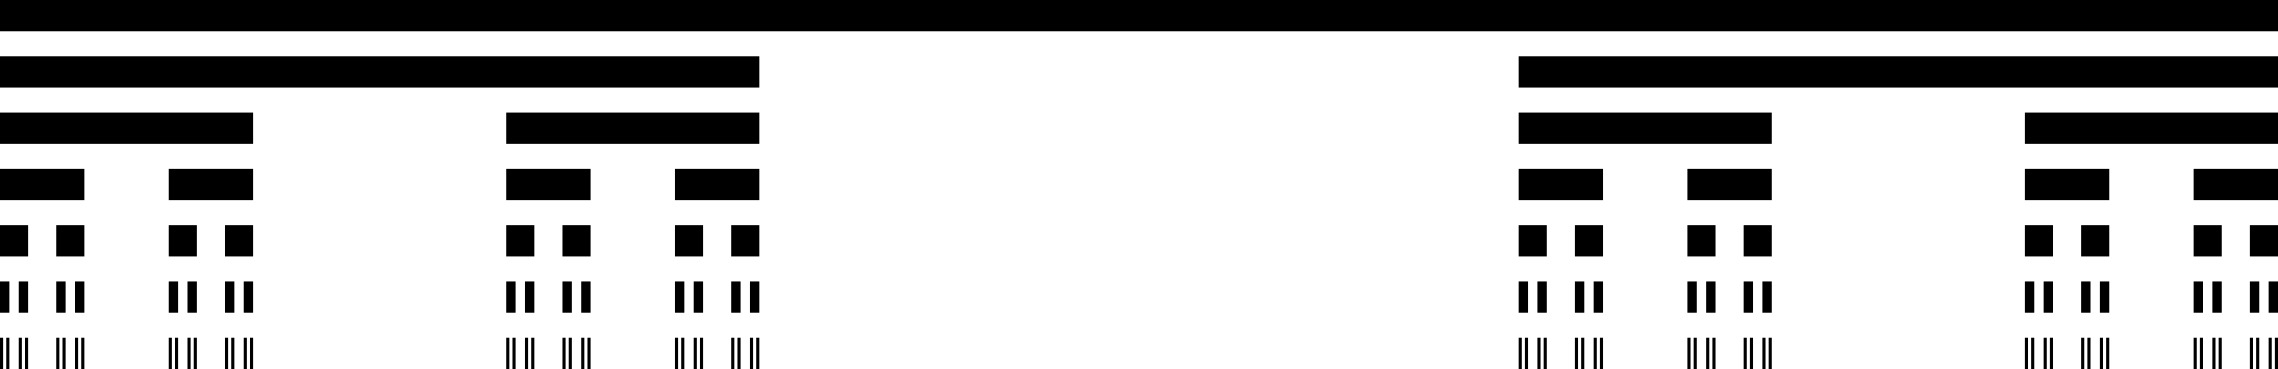
\includegraphics[width=0.8\textwidth]{Content/Images/Cantor_set_in_seven_iterations.jpg}
    \centering
    \caption{The first seven iterations of the middle third Cantor Set.}
\end{figure}
In a general sense, we can take a set, then dilate and translate a copy of it. 

\begin{definition}[Dilation]\cite{GEdgar}
    Let $r>0$ and $a \in \R$.  The \underline{dilation} on $\R$ with ratio $r$ and center $a$ is the function $f: \R \to \R$ given by $$f(x)= rx + (1-r) a.$$
\end{definition}

Now we consider the following two dilation funcitons each with the contraction ratio 1/3: 
$$f_1 (x) = \frac{1}{3}x \quad \text{ and } \quad f_2 (x) = \frac{x+2}{3}.$$


We will use these two to demonstrate that the Cantor set is self-similar.  This is an example of the definition of self similar, the collection of invariant points under iterated function systems.  In this case the two functions are the iterated funciton system and the set of invariant points is the Cantor set.  Admittedly this is an abstract definition so here is a proposition to work through the specific mechanics.  

\begin{proposition}The Cantor set is self-similar.   That is to say the Cantor set satisfies the self-referential equations 
    $$\mathcal{C} = f_1 [\mathcal{C}] \cup f_2 [\mathcal{C}].$$
\end{proposition}
\begin{proof}
    Recall the definition of the Cantor set, as the iterated removal of the middle third.      
    $$\mathcal{C} = [0,1] \setminus \bigcup_{n=0}^\infty\bigcup_{k=0}^{3^n-1}\left(\frac{3k+1}{3^{n+1}},\frac{3k+2}{3^{n+1}}\right)$$

    Here we notice that for the first removal, $n = 0$, we are left with the left and right portion of the Cantor set.  Specifically the left side is a translated copy of the right side:

    \begin{align*}
        \left[\frac{2}{3},1\right] \setminus \bigcup_{n=1}^\infty\bigcup_{k=0}^{3^n-1}\left(\frac{3k+1}{3^{n+1}},\frac{3k+2}{3^{n+1}}\right) &= \underbrace{ \left\{\left[0,\frac{1}{3}\right] \setminus \bigcup_{n=1}^\infty\bigcup_{k=0}^{3^n-1}\left(\frac{3k+1}{3^{n+1}},\frac{3k+2}{3^{n+1}}\right)\right\} }_{\text{the left side of the cantor set}}  + \frac{2}{3}\\
        &= \underbrace{ \frac{1}{3}\left\{[0,1] \setminus \bigcup_{n=0}^\infty\bigcup_{k=0}^{3^n-1}\left(\frac{3k+1}{3^{n+1}},\frac{3k+2}{3^{n+1}}\right)\right\} }_{\text{the left side of the cantor set}}  + \frac{2}{3} \\
        &= \frac{1}{3}\left\{ \underbrace{ [0,1] \setminus \bigcup_{n=0}^\infty\bigcup_{k=0}^{3^n-1}\left(\frac{3k+1}{3^{n+1}},\frac{3k+2}{3^{n+1}}\right) }_{\text{the original Cantor set}} \right\}   + \frac{2}{3} \\
        &=f_2 [\mcC] 
    \end{align*}

    We note that this happens at every level of the cantor set.  In otherwords by induction:
    $$\mcC_{n+1} = f_1[\mcC_n] \cup f_2 [\mcC_n].$$

    Notice that by using the above two equations, the Cantor set satisfies the self-referential equations:
    $$\mathcal{C} = f_1 \mathcal{C} \cup f_2 \mathcal{C}.$$


\end{proof}
\begin{definition}[Iterated Function System]
    An iterated function system is a finite set of contraction mappings on a complete metric space.  Symbolically, we write this as, for some $N \in \N$,
    $$\{f_i:X \to X \vert i = 1,2,\dots, N\}, $$
\end{definition}

\begin{definition}[Self-Similar Set]
    A set $A$ is self-similar if it is the invariant set of an iterated function system. 
\end{definition}


The invariant set under this iterated function system is a self similar set.
\section{An Erd\H{o}s Self\hyphen{Similarity} Conjecture in Measure Space}
    %History/Context for Erdos Conjecture, 
        %Proposed Year (1974)
        %Who are main researchers? 
        %Steinhaus: Finite sets are universal (predate Erdos)
        %Falconer(slow decay sequence, ratio test), 
        %Kolo
        %Bourgain: Faster decay sequences
        %What is current Progress?
        %Falconer(slow decay sequence, ratio test), 
        %Kolountzakis using probabilistic arguments
        %2^{-n} is still an open question
There is a long standing conjecture from Paul Erd\H{o}s on universal sets.  Informally the conjecture states that there is no infinite set that is universal in the real number line.  This is a conjecture about which types of  patterns can exist within another sets of numbers.  


We can now start by defining \textit{affine transformations} or \textit{affine copies}.
\begin{definition}[Affine copy]
    An \underline{affine copy} of a set $A \subset \R$ is a scaled and translated set $A'$ such that for some $\lambda\neq 0, \lambda \in \R$ and $t \in \R$,  $$A' = \{\lambda a + t : a \in A\}.$$
\end{definition}

In this instance, it is a scaled and then translated copy of the set is still one dimensional and therefore need not be a ``shape".  This gives us some flexibility when addressing different sets.  This definition is used to define measure universal. 

\begin{definition}[Measure Universal]
    A set $E$ is called \underline{measure universal} in $X$ if for every subset $S \subseteq X$, with positive measure, $\mu (S) > 0$, there exist an affine copy of $E$ such that $t+\lambda E \subseteq S,$ for some $\lambda \neq 0$ and $t \in \R$.  
\end{definition}

Now we can formally, state Erd\H{o}s' conjecture as follows. 

\begin{conjecture}[The Erd\H{o}s Similarity Conjecture]\label{ErdConj}
    Let $E\subseteq \R$ be an infinite set of real numbers.  Prove that there is a set of real numbers $S$ of positive measure which does not contain an affine copy of $E$.  
\end{conjecture}

Paul Erd\H{o}s originally posed this question back in 1974 by building off of the work of Steinhaus.  Steinhaus\cite{Steinhaus} first posed that finite sets are universal in sets with positive measure.  After Erd\H{o}s build on this with his conjecture, there has been some progress.

Later Falconer \cite{Falconer} made a substantial progress by showing slowly decaying sequences are not measure universal.  Bourgain \cite{Bourgain} expanded on this by showing some faster decaying sequences are also not measure universal.  In particular he demonstrated that the sum-set of any three sets, cannot be measure universal.  Most recently Kolountzakis \cite{Kolo} demonstrated using probabilistic arguments to demonstrate that certain set with large gaps cannot be measure universal.  

Currently it is still an open question whether or not sequences that decay at the rate of $2^{-n}$ are measure universal. 


In this paper we take this idea of measure universality and put it into a topological context.  We show in theorem \ref{theorem_positive_NW} no cantor set with positive Newhouse thickness is universal in the set of dense $G_\delta$ sets.


% \begin{conjecture}
%     There is no infinite universal set. 
% \end{conjecture}


\section{An Analogous Theorem in a Topological Setting}

In a non-rigorous exploration of the real numberline, one might assume that patterns which appear everywhere should have positive measure.  However density and measure are not intrinsically linked.  Indeed it is possible to have uncountable dense sets with measure zero and to have sets with full measure that are nowhere dense.  

Borrowing the conept of $G_\delta$ sets from topology, we can explore an extension of the Erd\H{o}s similarity problem.  Instead of exploring sets with positive measure we can explore dense $G_\delta$ sets.  This is the countable intersection of open sets that are also dense.  We will use these dense $G_\delta$ sets to define topological-universal. 

\begin{definition}[Topological-Universal]
    A set $E$ is called \underline{Topological-universal} in $\R$ if for every dense $G_\delta$ subset $S \subseteq \R$, there exist an affine copy of $E$ such that $t+\lambda E \subseteq S,$ for some $\lambda \neq 0$ and $t \in \R$.  
\end{definition}

As stated above, a dense $G_\delta$ set can have measure zero.  This also means that there is not a direct relationship between topological universal and measure universal.  We make two observations on this fact: a set with an interior cannot have be topologically universal, by the Baire Category Theorem all countable sets are topologically universal.   

This motivates the quesion, Is a nowhere dense set, with an empty interior topologically universal?  Cantor sets for example, have an empty interior and are nowhere dense.  

In chapter 2 we review background definitions and theorems in measure theory and topology.  We also give several examples to demonstrate some of the nuances of these facts.  In chapter 3 we define Newhouse Thickness, prove the Gap Lemma and prove our main result theorem \ref{theorem_positive_NW}.

\begin{theorem*}
Let $J$ be a cantor set with positive Newhouse thickness.  Then $J$ is not topologically universal.
\end{theorem*}

These results can also be extrapolated into $\R^d$ by definining projective Newhouse thickness.  Finally in chapter 4 we conclude with some open questions and remarks.  
% From these

% We have the new result that any Cantor sets with positive Newhouse thickness is not topologically universal.  We also conjecture that all cantor sets are not topologically universal.   


\chapter{Measure \& Topology}
\section{Some Measure Theoery}

First we want to begin with background definitions and theorems.  Erd\"{o}s' problem specifically deals with infinite set, and affine copies found in measurable set of sets.  In our problem, rather than dealing with measurable sets, we will instead use the set of dense $G_\delta$ sets.  

Underpinning the nuances of this problem, measure theoretic size, and topological size, are not the same. From an intuitive sense of the number line one might think when you are scattered throughout an interval, you would have measure, except in special cases. Similarly one might think that if you have measure, then you would be scattered everywhere.  However both of these instances fail when you add in rigorous arguments.  Indeed it is possible to construct a set that is no-where dense and have positive measure.  It is also possible to construct an uncountable set that is be dense and has zero measure. In other words topological size (density) is not the same thing as measure theoretic size. 

First we will review some measure theory.  In order to define \textit{measure} and \textit{measurable sets} we first need to define $\sigma$\hyphen{Algebra.   



\begin{definition}[$\sigma$-Algebra]
    Let $X$ be some set and $2^X$ be the set of subsets of $X$. Let $\Sigma \subseteq 2^X$. We call $\Sigma$ a $\sigma-$algebra over $X$ if it satisfies the following three conditions:
    \begin{enumerate}
        \item $\emptyset \in \Sigma$
        \item If $E \in \Sigma$, then $X\setminus E \in \Sigma$. 
        \item If $E_1, E_2, \dots \in \Sigma$ is a sequence of subsets, then $\bigcup_{k=1}^\infty E_k \in \Sigma$. 
    \end{enumerate}
\end{definition}

In this instance we describe set of sets in terms of inersection and union.  This allows us to generate an algebraically closed colleciton of sets.  Now if we have a base definition of measure, we are also able to contruct our colleciton of sets, on which measure is defined.   

\begin{definition}[Measure]
    Let $X$ be a set and $\Sigma$ be a $\sigma-$algebra over $X$.  A function $\mu: \Sigma \to \{\R \cup \infty\}$ is called a measure if it satisfies the following properties:
    \begin{enumerate}
        \item \textbf{Non-negativity}: for all $E \in \Sigma$, $\mu(E)\geq 0$.
        \item \textbf{Null empty set}: $\mu(\emptyset) = 0$. 
        \item \textbf{Countable Additivity} ($\sigma$-additivity): For all countable collections $\{E_k\}_{k=1}^\infty$ of pairwise disjoint sets in $\Sigma$, $$\mu\left( \bigcup_{k=1}^\infty E_k \right) = \sum_{k=1}^\infty \mu(E_k).$$
    \end{enumerate}
\end{definition}

In this instance, a measurable set 
\begin{definition}[Measurable Set]
    Let $(X,\Sigma)$ be a measurable space.  A set $S\subseteq X$ is a \textit{measurable set} if and only if $S \in \Sigma$.
\end{definition}
Note that a non-measurable set is a set that is not in the $\sigma$-algebra.  That is to say not all sets are necessarily measurable.  Nonmeasurable sets fall outside of our work.  

%Need to define Lebesgue measure


We will also need to define \textit{uncountable} and \textit{dense}.  First we start with \textit{countable}.

\begin{definition}[Countable]
    A set $X$ is called \textit{countable} if for some  subset $N \subset \N$, that is not necessarily finite, there exists a bijection $f: X \to N$.  
\end{definition}

\begin{definition}[Uncountable]
    A set $X$ is called \textit{uncountable}, if it is not \textit{countable}.
\end{definition}

We also need to define \textit{dense}.  There are many equivalent definitions of dense.  We will use the following definition so that we can continue to develop the intuion around intervals and interiors. 

\begin{definition}[Dense]
    A set $S$ is called dense in $X$ if for every $x \in X$, every neighborhood $U$ of $x$ intersects $A$.  
\end{definition}


In a similar fashion to the definitions of \textit{countable} and \textit{uncountable}, the oppsite of \textit{dense} is \textit{nowhere dense}.

\begin{definition}[Nowhere Dense]  Let $X$ be a topological space.  A subset $B \subseteq X$ of a topological space is called \textit{nowhere dense} in $X$ if its closure has an empty interior.  That is to say, $B$ is \textit{nowhere dense} in $X$ if for each open set $U\subseteq X$, $B\cap U$ is not dense in $U$.      
\end{definition}


This allows us to now explore the differences between density and measure.  As stated earlier, topological size and measure theoretic size are not necessarily related.  What do we mean by topologically Large? Uncountable and dense.  Similarly what do we mean by measure theoretically large?  Non-zero measure.  After reviewing t It is helpful to define the opposite of topologically large, namely meager sets.



\begin{definition}[Meager]  A subset $C \subseteq X$ of a topological space is called \textit{meager} in $X$ if it is the countable union of nowhere-dense subsets of $X$.    
\end{definition}
Now we look at our example.  
\begin{example}A measure theoretically large set is not necessarily topologically large.

Consider the interval $[0,1]$ and for all positive integers $a,n \in \N$ remove the intervals $(\frac{a}{2^n} - \frac{1}{2^{n+1}},\frac{a}{2^n} + \frac{1}{2^{n+1}})$.  Notice that the intervals are a geometric series and for each $n$ add up to at most $\frac{1}{2^{n+1}}$.  Therefore the set 
$$[0,1] \setminus \bigcup_{a,n \in \N} \left(\frac{a}{2^n} - \frac{1}{2^{n+1}},\frac{a}{2^n} + \frac{1}{2^{n+1}}\right),$$
is closed, has an empty interior, and is of positive measure.  
\end{example}

Next we will define dense $G_\delta$ sets, as well as some useful examples.  
\begin{definition}[G-Delta Set]
    A $G_\delta$ set is the countable intersection of open sets.  Namely, let $O_i \subset X$ for $i \in \N$ be a collection of open sets of $X$.  Then 
    $\bigcap_{n=1}^\infty O_i,$ is a $G_\delta$ set.  
\end{definition}

\begin{example}
    The irrational numbers are a $G_\delta$ set.  Consider the following construction of the set of irrational numbers:
    $$\R \setminus \Q = \bigcap_{q \in \Q}\R \setminus \{q\}.$$
\end{example}
Notice that each $\R\setminus \{q\} = (-\infty, q) \cup (q, \infty)$ is an open subset of $\R$.  Furthermore, rational numbers are countable.  Therefore the intersection of these sets are a $G_\delta$ set.  Moreover, in this instance it is a dense $G_\delta$ set.  We will study these objects further.  

Lastly we remark that there is an analogous set which is the countable union of closed sets.
\begin{definition}[F$_\sigma$ Set]
    An $F_\sigma$ set is the countable union of closed sets.  This is equivalent to the compliment of a G-delta is an F-sigma set.  
\end{definition}

%measure big topological small
%topologically big (dense g_delta), measure small 
\section{Cantor Sets and Other Measure Theoretic and Topological Examples}
We begin this section with a special $F_\sigma$ set.  The Cantor set is defined by taking the interval $[0,1]$ and then iterate by removing the open interval containing the middle third, from the previous level.  As such it is the countable intersection of closed sets.  Formally this can be written as follows.
\begin{definition}[Cantor Set]
    The Cantor set $\mathcal{C}$, written as the successive removal of each middle third removed from the previous level is 
    $$\mathcal{C} = [0,1] \setminus \bigcup_{n=0}^\infty\bigcup_{k=0}^{3^n-1}\left(\frac{3k+1}{3^{n+1}},\frac{3k+2}{3^{n+1}}\right)$$
\end{definition}

As an $F_\sigma$ set defined on a closed interval with iteratively removed open intervals we see the middle third Cantor set can also be described with the following three properties.
\begin{definition}[Cantor Set]
    \textit{Cantor sets} are compact, perfect sets, and totally disconnected sets.      
\end{definition}

As a quick reminder to the definitions:
\begin{definition}[Perfect]
    A \textit{perfect} set is a closed set that contains no isolated points.
\end{definition}
\begin{definition}[Totally Disconnected]
    A set is \textit{totally disconnected} if the only connected components are single points. 
\end{definition}


An equivalent formulation of the Cantor set, is the decimal expansion of all numbers in $[0,1]$ in base $3$, omitting any representation with a $1$. This can be a useful tool for thinking through some examples and counter-examples.
\begin{example}[Decimal Expansion Cantor Set]
    $$\mathcal{C}  = \{ x \in [0,1]: \text{ $x$ has a ternary expansion containing no $1$'s.}\}$$
\end{example}
Here we notice that although $1/3 \in \mathcal{C} $ can be written as $0.1$ using the ternary expansion, it also has another representation as $1/3 = 0.0\overline{2}$  This would be the included representation in the Cantor set.  We take a moment to acknowledge that numbers may not have unique representations, where one may be excluded but the other included.  

Earlier we defined nowhere dense. Here we see that the Cantor set is an example of a nowhere dense set.  
% \begin{definition}[Nowhere dense]
%     A set $A \subseteq X$ is called \textit{nowhere dense} if its closure $\overline{A}$ has an empty interior.  Equivalently the set $A$ is \textit{nowhere dense} if $A$ is not not dense in any subset $U$ of $X$.  
% \end{definition}
\begin{claim}The Cantor set is \textit{nowhere dense}.  
\end{claim}  
\begin{proof}
    Let $\mcC$ be the middle third Cantor set.  Notice that $[0,1]\setminus \mcC$ is a set of open intervals: 
    $$ [0,1] \setminus \mathcal{C} =\bigcup_{n=0}^\infty\bigcup_{k=0}^{3^n-1}\left(\frac{3k+1}{3^{n+1}},\frac{3k+2}{3^{n+1}}\right). $$
    Therefore $\mcC$ is the countable intersection of closed intervals, and itself is closed.  
    
    Notice given some radius $r$, there exists some number $t$, such that $0<t<r$ and $t$ has a 1 in its ternary expansion.  So if we consider any point $c \in \mcC$, then an open ball of radius $r$ centered at $c$ then $B_r(c)$ is $(c-r, c+r)$ in ternary, necessarily contains a number containing a $1$.  Therefore $B_r(c) \not\subseteq \mcC$, and $\mcC$ has an empty interior.  Finally we conclude because $\mcC$ is closed and has an empty interior, $\mcC$ is nowhere dense.      
\end{proof}
Beyond the middle third Cantor set, we can generalize these in a few different ways.  Changing the middle interval, having a few different interval widths, series of interval widths. 
%\begin{definition}{Generalized Cantor's Set}
%    Middle Third Cantor Set
%\end{definition}

\begin{figure}
    \begin{center}
    
\begin{tikzpicture}
%\draw (-1,.5) -- (28, .5);
% \draw [(-)](9,0) -- (18, 0);
%\draw (-1,0) -- (28, 0);
%\draw (-1,-.5) -- (28, -.5);
%\draw (-1,-1) -- (28, -1);
%\draw (-1,-1.5) -- (28, -1.5);
\draw [line width = 1.5mm] (0,.5) -- (9, .5);
\draw [decoration=Cantor set,line width =1.5mm] decorate{ (0,0) -- (9,0)};
% \draw [(-)](9,0) -- (18, 0);
\draw [decoration=Cantor set,line width =1.5mm] decorate{ decorate{ (0,-.5) -- (9,-.5) }};
\draw [(-)](3,0) -- (6, 0);
% \draw [(-)](21,-0.5) -- (24, -0.5);
\draw [decoration=Cantor set,line width =1.5mm]decorate{ decorate{ decorate{ (0,-1) -- (9,-1) }}};
\draw [(-)](1,-0.5) -- (2, -0.5);
\draw [(-)](7,--0.5) -- (8, --0.5);
% \draw [(-)](19,-1) -- (20, -1);
% \draw [(-)](25,-1) -- (26, -1);
\draw [decoration=Cantor set,line width =1.5mm] decorate{ decorate{ decorate{ decorate{ (0,-1.5) -- (9,-1.5) }}}};
\draw [(-)](1/3,-1) -- (2/3, -1);
\draw [(-)](7/3,-1) -- (8/3, -1);
\draw [(-)](19/3,-1) -- (20/3, -1);
\draw [(-)](25/3,-1) -- (26/3, -1);
\end{tikzpicture}
\end{center}
\caption{The open middle intervals are recursively removed.  This removes the interior of the set, while still leaving the original set closed.  }
    \label{fig:my_label}
\end{figure}


\begin{example}[A measure theoretically large set is not necessarily topologically large.]
    The Smith-Volterra-Cantor set is formed in a similar manor to the middle-third Cantor set.  Starting with the closed interval, remove the middle fourth recursively.  At each level, $2^{n-1}$ intervals of length $1/4^n$ are removed.  The total length of these removed intervals are $$\sum_{n=0}^\infty \frac{2^n}{2^{2n+2}} = \frac{1}{2}.$$
    Therefore the Smith-Volterra-Cantor set has measure $1 - 1/2 = 1/2.$
    This closed set still has an empty interior and is therefore nowhere dense but still has positive measure. 
%Consider the interval $[0,1]$ and for all positive integers $n \in \N$ remove the intervals $(\frac{1}{2^n} - \frac{1}{2^{n+1}},\frac{a}{2^n} + \frac{1}{2^{n+1}})$.  Notice that the intervals are a geometric series and for each $n$ add up to at most $\frac{1}{2^{n+1}}$.  Therefore the set 
%$$[0,1] \setminus \bigcup_{a,n \in \N} \left(\frac{a}{2^n} - \frac{1}{2^{n+1}},\frac{a}{2^n} + \frac{1}{2^{n+1}}\right),$$
%is closed, has an empty interior, and is of positive measure.  
\end{example}

\begin{example}[A dense, uncountable set of measure zero]
As stated above, the middle third Cantor set has measure $0$.  Let $\mcC_q$ denote a cantor set translated by a rational number $q \in \Q$.  This gluing of sets is dense but still measure zero.  This is formed from closed sets. 
$$\left\vert \bigcup_{q \in \Q} \mcC_q \right\vert \leq  \sum_{q \in \Q}\left\vert\mcC_q\right\vert = 0.$$
\end{example}

\section{The Baire Category Theorem}
A key theorem that links analysis to set theory is the Baire Category Theorem.  This also establishes a link to understanding certain types of topological sets.  
\begin{theorem}[Baire Category Theorem]
    The countable intersection of open dense sets is dense.  
\end{theorem}

Within the study of measure theory it can sometimes be unclear if a set is dense in another set.  For example consider the following set: 
$$\R^2 \setminus \{(x,y): y=mx + b, \text{where $m, b \in \Q$.}\}$$
Notice that this can also be written as $$\bigcap_{m,b \in \Q} \R^2 \setminus \{(x,y): y=mx+b\}, $$ which is the plane, but removing all lines with rational coefficients, and rational intercepts.  
%\chapter{An Erd\"{o}s Conjecture in Measure Theory}

\chapter{An Erd\"{o}s Similarity Problem in a Topological Setting}
\section{Positive Newhouse Thickness}
Cantor sets contain important invariant structures such as Hausdorff dimension, thickness, and denseness.  We will investigate thickness and denseness.  First we will define the gaps and bounded gaps of Cantor sets in order to construct and define Newhouse thickness. 

The Gap lemma was originally interoduced by Newhouse in his paper "The Abundance of Wild Hyperbolic Sets and Non-Smooth Stable Sets for Diffeomorphism," \cite{Newhouse}.  This lemma proves useful in dynamical systems.  Our lemma is borrowed from Palis and Takens "Hyperbolicity \& Sensitive Chaotic Dynamics at Homoclinic Bifurcations."  There has also been additional work by Astels, where in his disseration \cite{Astels} he details the structure of the intersections.  
\begin{definition}[Gap]
    Let $K$ be some Cantor set.  A \textit{gap} of $K$ is a connected components of $\R \setminus K$.      
\end{definition}  Informally, the gaps are the intervals surrounding the points of the Cantor set.  Some of the lengths of these intervals are bounded some are not.  In the example of the middle third Cantor set, the unbounded gaps would be $(-\infty, 0)$ and $(1, \infty)$.  

\begin{definition}[Bounded Gap]
    Let $K$ be a Cantor set.  A \textit{bounded gap} is a bounded connected component of $\R \setminus K$.      
\end{definition}

Using these two notions we will define the \textit{bridge} of $C$ of Cantor set $K$.  
\begin{definition}[Bridge]\cite{palis&takens}
    Let $K$ be some cantor set and $U$ be a bounded gap of $K$ with boundary point $u$.  The \textit{bridge} $C$ of $K$ at $u$ is the maximal interval in $\R$ such that:
    \begin{itemize}
        \item $u$ is a boundary point of $C$
        \item $C$ contains no point of a gap $U'$ whose length $\ell(U') \geq \ell(U)$..
    \end{itemize}
\end{definition}

For clarity the picture below shows that there may be smaller bounded gaps contained in $C$.  

\vspace*{0.25cm}
% \begin{figure}
% \centering
\begin{tikzpicture}
    \draw (-6.5,0) -- (6.5,0) ;
    \draw[(-)] (-5,0)--(-3,0);
    \draw[very thick] (-5,0) --  (-3,0) node[midway, above]{$U$} node[below]{$u$};
    \draw[(-)] (-2,-1)--(-1.25,-1)node[midway, below]{$U_1$};
    %\draw[very thick] (0.92,0) -- (1.92,0);
    \draw[(-)] (0.5,-1) -- (1.75,-1)node[midway, below]{$U_2$};
    \draw[(-)] (3,0)--(6,0);
    \draw[very thick] (3,0) -- (6,0)node[midway, above]{$U'$};
    \draw[below,{[-]}]  (-3,-0.75) -- (3,-0.75) node[midway, above]{$C$};
    \draw[very thick]  (-3,-0.75) -- (3,-0.75);
\end{tikzpicture}
% \end{figure}

We use this notion to define the \textit{Newhouse Thickness}.  Intuitively the thickness of a Cantor set can be thought of as a the infimimum of ratios between the bounded gaps and the bridges.  
\begin{definition}[Newhouse Thickness \cite{palis&takens}]
    The \textit{Newhouse Thickness or thickness of $K$ at $u$} is defined as
    $$\tau(K, u) = \frac{\ell(C)}{\ell(U)}.$$
    Moreover for $\mathcal{U} = \{ \text{set of all boundary points of bounded gaps}\}$, the thickness of the entire Cantor set is 
    $$\tau(K) = \inf_{u\in \mathcal{U}} \tau(K, u) = \inf_{u\in \mathcal{U}}\frac{\ell(C)}{\ell(U)}$$
\end{definition}
This helps us develop a language to talk about the relative sizes of Cantor sets that is slightly separated from the notion of measure.  Importantly it also helps us for a sufficient condition for our main theorem.

Here we will calculate a few examples of Newhouse Thickness.  Recall the middle third Cantor set.  
\begin{example}[Newhouse Thickness of the Middle\hyphen{third} Cantor Set]
    Let $K$ be the middle third cantor set.  Then the Newhouse thickness is the infimum of the ratio between gaps and bridges.  Here we notice that every bounded gap is one third the previous bridge.  Therefore the Newhouse thickness of the set is 
    $$\tau(K) = \inf_{u\in K}\frac{\ell(C)}{\ell(U)} = \frac{\frac{1}{3}}{\frac{1}{3}} = 1.$$
\end{example}

\begin{example}[Newhouse Thickness of the $N$\hyphen{digit} Cantor Set]
    Let $K$ be an $N$\hyphen{digit} Cantor set.  Each gap at the $n$\hyphen{th} level is of has length $N^{-n}$.  We take a moment to note that the location of the gap matters because it affects the thickness.  If we assume that for $2 \leq j \leq n-1$, the $j$\hyphen{th} digit is removed then we end up with the following cantor set. 
    % Damn I drew the wrong pictures... should have just copied from above.
    % \begin{tikzpicture}
    %     \draw (-7,-0.75) -- (7,-0.75) ; %total length 14
    %     \draw (-7,-1.75) -- (7,-1.75) ; %total length 12
    %     \draw[{[-]}] (-6,-0.75)--(-2,-0.75); %sub length 4
    %     \draw[ultra thick] (-6,-0.75) --  (-2,-0.75) node[midway, above]{$C_i$} node[above]{$j_i$}; %left side
    %     \draw[(-)] (-2,-1)--(-1,-1)node[midway, below]{$U_i$}; %bdd gap
    %     \draw[(-] (5,-1)--(7,-1)node[midway, below]{$U_{i+1}$}; %bdd gap
        
    %     \draw[{[-]}]  (-1,-0.75) -- (5,-0.75) node[midway, above]{$C_{i+1}$};%sublength 7
    %     \draw[ultra thick] (-1,-0.75) -- (5,-0.75); %right side

    %     %left, scaled by 1/4
    %     \draw[{[-]}] (-6,-1.75) -- (-5,-1.75);%node[midway, below]{$C_{i+2}$};
    %     \draw[very thick] (-6,-1.75) -- (-5,-1.75);
    %     \draw[(-)] (-5,-2)-- (-4.75,-2);%node[midway, below]{$U_{i+1}$};
    %     \draw[{[-]}] (-4.75,-1.75)--(-2,-1.75) ;%node[midway, below]{$C_{i+3}$};
    %     \draw[very thick] (-4.75,-1.75)--(-2,-1.75);
    %     \draw (-5.5,-2.25)node{$\vdots$};
    %     \draw (-3.25,-2.25)node{$\vdots$};    
        
    %     %right scaled by 1/7 +5
    %     \draw[{[-]}]  (-1,-1.75) -- (6/7,-1.75);% node[midway, below]{$C_{i+4}$};
    %     \draw[very thick] (-1,-1.75) -- (6/7,-1.75);
    %     \draw[(-)] (6/7,-2)-- (6/7+7/12,-2) ;%node[midway, below]{$U_{i+2}$};
    %     \draw[{[-]}] (6/7+7/12,-1.75)--(5,-1.75) ;%node[midway, below]{$C_{i+5}$};
    %     \draw[very thick] (6/7+7/12,-1.75)--(5,-1.75);
    %     \draw (-1/14,-2.25)node{$\vdots$}; 
    %     \draw (2.5+3/7 +7/24,-2.25)node{$\vdots$}; 
    % \end{tikzpicture}

%the right picture...
    \begin{tikzpicture}
        \draw (-6.5,0) -- (6.5,0) ;
        \draw[(-)] (-5,0)--(-3,0);
        \draw[very thick] (-5,0) --  (-3,0) node[midway, above]{$\frac{1}{N^n}$} node[below]{$u$};
        \draw[(-)] (-2,-1)--(-1.25,-1)node[midway, below]{$U_1$};
        %\draw[very thick] (0.92,0) -- (1.92,0);
        \draw[(-)] (0.5,-1) -- (1.75,-1)node[midway, below]{$U_2$};
        \draw[(-)] (3,0)--(6,0);
        \draw[very thick] (3,0) -- (6,0)node[midway, above]{$U'$};
        \draw[below,{[-]}]  (-3,-0.75) -- (3,-0.75) node[midway, above]{$C$};
        \draw[very thick]  (-3,-0.75) -- (3,-0.75);
    \end{tikzpicture}

    With this picture in mind lets take the infimum of the ratios.  The thickness of the $N$\hyphen{digit} expansion Cantor set is 
    $$\tau(K) = \inf_{u\in K}\frac{\ell(C)}{\ell(U)} = \min\left\{j,N-j-1\right\}$$
\end{example}  
%include examples of calculating newhouse thickness
%Cantor set Middle Third
%N Digit
%Comment on removing left interval doesn't work well.  Thin left interval versus Thick Right interval
%Also note that all self-similar Cantor sets in \R^1 have positive newhouse thickness
\section{The Gap Lemma}
\begin{lemma}[The Gap Lemma\cite{palis&takens}]
    Let $K_1, K_2, \subset \R$ be Cantor sets with thickness $\tau_1$ and  $\tau_2$.  If $\tau_1 \cdot \tau_2 >1,$  $K_1$ is not contained the gap of $K_2$, $K_2$ is not contained in the gap of $K_1$ then $K_1 \cap K_2 \neq \emptyset.$
\end{lemma}
% First we will assume for the sake of contradiction that the opposite is true.  These assumptions lead to claim, which under these assumptions must be true.  Then that claim leads to a contradiction which means our original assumption must be false.  
\begin{proof}
    Let $K_1, K_2$ be two Cantor sets with thickness $\tau_1, \tau_2$ respectively such that $K_1$ is not contained in the gap of $K_2$ and $K_2$ is not contained in the gap of $K_1$.  

    Assume for the sake of contradiction that $K_1 \cap K_2 = \emptyset$.  Consider the bounded gaps $U_1 \subset K_1^c$ and $U_2 \subset K_2^c$.  We call $(U_1, U_2)$ a gap-pair if $U_1$ contains exactly one boundary point of $U_2$ and $U_2$ contains exactly one point of $U_1$.  

    We want to use this technique to demonstrate that $K_1 \cap K_2 \neq \emptyset.$ Let $C_j^l, C_j^r$ denote the bridges of $K_j$ for $j = 1,2$.  Returning to our original assumptions, $\tau_1 \cdot \tau_2 > 1$ and therefore $$\frac{\ell(C_1)}{\ell(U_2)} \cdot \frac{\ell(C_2)}{\ell(U_1)} > 1.$$  
    %If $q \not\in K_1,$ then $q \in U_1'$, 
    The gap of $K_1$ where $\ell(U_1') < \ell(U_1)$ and $(U_1', U_2)$ is the gap pair we need.  
    
    From our construction, the right endpoint of $U_2$ is in $C_1^r$ or the left endpoint of $U_1$ is in $C_2^l$ or both.  By assumption we know that $K_1, K_2$ are not contained in the other's gaps. Therefore there exists some gap-pair $(U_1, U_2).$

    %In the case that $q \in U_2$ is the right endpoint, then $q \in K_1$ and $q \in K_2$ and we are done.  

    A quick picture can help show where these pieces are located:  This picture is not accurate because we are using this to derive a contradiction.
    
    \begin{tikzpicture}
        %First Cantor Set K_1
        \draw (-6.5,0) -- (6.5,0) ;
        \draw[(-)] (-5,0.25)--(-3,0.25) node[midway, above]{$U_1$};
        \draw[below,{[-]}]  (-3,-0.75) -- (3,-0.75) node[midway, above]{$C_1$};

        %second cantor set K_2
        \draw[{[-]}] (-6,0) --  (-4,0) node[midway, below]{$C_2$};
        \draw[(-)] (-4,-1)--(-1.25,-1)node[midway, below]{$U_2$};
        \draw (-6.5,-0.75) -- (6.5,-0.75) ;
    \end{tikzpicture}
    \begin{claim}
        If $\tau_1\tau_2 > 1$ then from the interval $U_1$ (or for that matter $U_2$) we can construct another sub-interval $U_1'$ such that $\ell(U_1') < \ell(U_1)$ (or similarly $U_2'$ such that $\ell(U_2')<\ell(U_2)).$
    \end{claim}
    %Proof of claim
    Notice that $(U_1',U_2)$ is still a gap-pair, as is $(U_1,U_2')$.
    
    Using this construction we can create a sequence of gap-pairs $(U_1^{(i)}, U_2^{(j)})$.  Notice that the sum is finite $$\sum_i^\infty \ell(U_1^{(i)}) < \infty,$$ and therefore $\ell(U_1^{(i)}) \to 0$ as $i \to \infty$.   From this we construction we have a sequence of gap-pairs such that as $i \to \infty$, $\ell(U_1^{(i)}) \to 0$ and similarly as $j \to \infty$, $\ell(U_2^{(j)}) \to 0$.  
    
    Without loss of generality, we can form a subsequence and use the same indexing for the gap pairs, $(U_1^{(i)}, U_2^{(i)})$.  
    
    This sequence of gap pairs have a non-empty intersection for all $i \in \N$.  

    Notice that by picking a sequence of points, $q_{i} \in U_1^{(i)}$ this forms a convergent subsequence $q_{i_k} \to q$.  Notice that $U_1^{(i)}$ 
    %= (a_i, b_i)$ 
    is not fully contained in the gap of $K_2$.  Moreover because these intervals are compact and nested, we know that %$a_{i_k} - b_{i_k} \to 0$ 
     $q$ which is contained in each $U_1^{(i)}$ is therefore in  $K_2$.  

    Because this construction is symmetric, the same argument applies to $q_{i} \in U_2^{(i)}$ and so $q \in K_2$.  Therefore the Cantor sets share at least one point, $q \in K_1 \cap K_2$.  

\end{proof}
\section{A Cantor set with positive Newhouse Thickness is not Topologically Universal}

Recall the definition, 
We  say that a set $E$ is  {\it topologically universal} in the collection of dense $G_{\delta}$ sets if for all $G_{\delta}$ set,  we can  always find some affine copies of $E$ inside the set. By an affine copy, we  mean sets of  the form $t+\lambda E$ for some $t\in{\mathbb R}$ and $\lambda\ne 0$. A natural question we have is that  is there a nowhere dense Cantor Set that is universal in the collection of dense $G_\delta$ sets? This is an exploration of an Erd\"{o}s conjecture in a topological setting. 

\begin{theorem}\label{theorem_positive_NW}
Let $J$ be a cantor set with positive Newhouse thickness.  Then $J$ is not topologically universal in the collection of dense $G_\delta$ sets.
\end{theorem}

\begin{proof} Suppose we have some Cantor set $J$ with Newhouse thickness $\tau(J) >0$. Without loss of generality, we  can assume  the convex hull of $J$ $[0,1]$.   Consider Cantor sets $K$ defined by contraction ratio $1/N$ and digits $\{0,1,...,N-1\}\setminus\{(N-1)/2\}$ and $N$ is odd. By a simple calculation,  $\tau (K) = \frac{N-1}{2}$. Therefore,  we can find a  sufficiently large $N$ so that $\tau(J)\tau(K)>1$. 

\medskip

Using the Cantor set $K$ Define $X$ such that $$
X = \bigcup_{n \in \Z} \bigcup_{\ell \in \Z} N^n(K+\ell),
$$creating a dense $F_\sigma$ set. Now consider $X^c$.  Because $K^c$ is open and dense and so is its translated and dilated copies, by the Baire Category Theorem, $X^c$ is a dense $G_{\delta}$.  We now show that $X^c$ contains no affine copy of $J$. 

\medskip

Suppose we have some affine copy, $t+ \lambda J$ where $t\in\R$ and $\lambda\ne 0$. There exists a unique $n$ such that 
\begin{equation}
    |\lambda| \in (N^{n-1}, N^n].
\end{equation}
Similarly there exists a unique $\ell$ such that 
\begin{equation}
t \in (\ell  N^n, (\ell+1)N^n].    
\end{equation}


%We claim that this affine copy of $J$ has a non-empty intersection with $N^n(K+\ell)$.  This is equivalent to  showing that 
%$$t \in N^n(K+\ell)-\lambda J.$$
Let 
$$C_1 = N^n(K+\ell) \text{ and } C_2 = t+ \lambda J.$$
The convex hull of $C_1,$ is  $[\ell  N^n, (\ell+1)N^n]$.  So By our choice of $t$, we know that $C_2$ is not in the unbounded gap of $C_1$ and vice versa.  

Now we will check the construction of our Cantor sets such that each is not contained in the bounded gaps of the other. For $C_1$ its largest corresponding open gap interval is $|O_1| = N^{n-1}$ and its largest corresponding closed interval is $|I_1| = N^n$. For $C_2$ and is corresponding intervals, we find that $|O_2| =|\lambda|\cdot |O_J| \le |\lambda|$ and $|I_2| = |\lambda|$ where $O_J$ is the largest  open gap interval in $J$.  Therefore by our construction in (1) the following two inequalities hold: $$|O_1|\leq |I_2| \text { and } |O_2| \leq |I_1|.$$ Therefore $C_1$ is not in the gaps of $C_2$ and $C_2$ is not fully contained in the gaps of $C_1$.  By our choice of K, the Newhouse thickness of our sets, $\tau(C_1))\tau(C_2) \geq 1$, because Newhouse thickness is scale invariant.  Therefore the the Gap Lemma implies $C_1 \cap C_2$ is non-empty and $C_2$ cannot be in the constructed $G_{\delta} $ set. Therefore we conclude $J$ is not topologically universal in the collection of dense $G_\delta$ sets.  


%as in the condition of Theorem 2.2.1 in \cite{Astels}.  By \cite [Theorem 2.2.1]{Astels}\footnote{This might misattribute the theorem.  I think Astels '99 Theorem 2.2.1 is  actually is quoting Newhouse directly.  In particular I think it refers to Newhouse 1979 \cite{PMIHES_1979__50__101_0} \textit{The Abundance of Wild Hyperbolic Sets, and Non-smooth Stable Sets for Diffeomorphisms}. }, given that the Newhouse thickness of our sets, $\tau(K)\tau(J) \geq 1$ then $C_1 + C_2 = I_1 + I_2$. Note that   $I_1 = [\ell N^n, (\ell+1)N^n]$,  $I_2=[-\lambda, 0]$ if $\lambda>0$  and $I_2=[0,-\lambda]$ if $\lambda<0$.  we find that 
% $$
% I_1+ I_2 = [N^n\ell - \lambda, N^n(\ell+1)] \  (\lambda>0) \ \mbox{and} \ I_1+I_2 = [N^n\ell, N^n(\ell+1)-\lambda] (\lambda<0).
% $$
% Then from (2)
% $$t \in I_1+I_2.$$
% Therefore the affine copy of the cantor set $t + \lambda J$ has a non-empty intersection with $X$ and $J$ cannot be universal.

\end{proof}

%It would be interesting to study those Cantor sets with Newhouse thickness zero. We do not  know what would happen. However, it seems like if we assume a weaker condition on $J$. 

\medskip

%\noindent $(\ast):$ There exists $K$ such that $J+K = I_J+I_K$, where $I_J,I_K$ are the  smallest closed interval containing $J$ and $K$. 

\medskip

%we  may be able to show that  $J$  cannot be  universal for dense $G_{\delta}$ sets. 

\section{Generalizing into Higher Dimensions}
%higher dimension, affine copy will be different in a few ways: \lambda, can be an orthogonal transformation, or scalar, t can be a vector.

Consider a compact set $J$ in $\R^d$. An affine copy of $J$ is $\R^d$ is the set 
$$
t+\delta O (J)
$$
where $t\in \R^d$, $\delta\ne 0$ and $O$ is an orthogonal transformation. We say that $J$ is universal is the collection of dense $G_{\delta}$ sets if any dense $G_{\delta}$ set contains an affine copy of $J$. 
%Falconer and Yavicoli generalize newhouse thickness to higher dimension, but their definition of thickness in higher dimension has to have a path connected component.  
\begin{theorem}
    If $X\subset \R^d$ contains a path connected component, then $X$ is not universal in the set of dense $G_\delta$ sets of $\R^d$.  
\end{theorem}
\begin{proof}
    Remove the plane 
    $$
    \R^d \setminus \bigcup_{i=1}^d \bigcup_{r \in \Q} \{X_i = r \}.
    $$
    This is clearly a dense $G_{\delta}$ set. 
    Consider any affine copy of $X$ must contain a path $L$.   The projection of $L$ onto the coordinate axes will be non-degenerate on some interval for at least one of the axes.  Call this the $i$-th axis.  This interval will contain a rational number $r$.  Therefore $L$ will intersect with the coordinate plane, $X_i = r$ 
    In other words this dense $G_{\delta}$ set omits at least one point and cannot contain affine copy of $X$.  
\end{proof}
 We can still consider sets that contain no connected component.  Cantor dust contains no connected component.  We introduce the notion of \textit{projective Newhouse Thickness}, and use it to generalize our one-dimensional results into $\R^d$.  
\begin{definition}[Positive Projective Newhouse Thickness]
    We say a $J$ set has {\it positive projective Newhouse thickness} if for all ${\mathcal O} \in O(d)$ 
$$
 \tau(P_x{\mathcal O}(J)) > 0
$$
where $P_x$ is the orthogonal projection to the $x$-axis and $O(d)$ is the orthogonal group consisting of all orthogonal transformations in ${\mathbb R}^d$.  
\end{definition}

We note that the projection some Cantor dust set maybe an interval.  If that is the case we say the Newhouse Thickness of the projection is equal to infinity.  

%remark or compute projective newhouse thickness.  

Using our one dimensional result, we can generalize 
\begin{theorem}Suppose $J \subset \R^d$ has positive projective Newhouse thickness. Then $J$ is not topologically-universal in $\R^d$.  
\end{theorem}

\begin{proof}  Suppose we have a set $J$ in $\R^d$ such that it has a positive projective Newhouse thickness. In Theorem \ref{theorem_positive_NW}, we can actually see that for all Cantor sets $J'$ with Newhouse thickness at least $\epsilon$, there exists the dense $G_{\delta}$ set  omits all affine copies of $J'$. Hence, we take $\epsilon = 1/n$,  there exists $G_n$, a dense $G_{\delta}$ set in ${\mathbb R}^1$ such that $G_n$ omits all affine copies of all cantor set $J'$, with $$\tau(J') \geq \frac{1}{n}.$$
    % $P_x O(J)$. 
Now, from these $G_n$ we construct
$$
G = \bigcap_{n=1}^\infty G_n\underbrace{\times \dots \times}_\text{d-times}G_n. 
$$
Each $G_n\underbrace{\times \dots \times}_\text{d-times}G_n $ is a dense $G_\delta$ set in ${\mathbb R}^d$ and therefore $G$ is also a dense $G_\delta$ set by the Baire Category theorem.  

Now all that remains is to prove that $G$ has no affine copy of $J$.   Assume to the contrary that $G$ contains an affine copy of $J$ and denote it by $t+\lambda \mathcal{O}J$. Note that the assumption implies that 
$$
\tau(P_x(t) + \lambda P_x\mathcal{O}(J)))> 0.
$$
Hence, there exists some $n$ so that the above thickness is at least $\frac{1}{n}.$ By our construction of $G_n$, $G_n$ has no affine copy of $P_x\mathcal{O}(J)$.  But if $t + \lambda \mathcal{O}J \subset G = \bigcap_{n=1}^\infty G_n \times \dots \times G_n,$ then $t+\lambda \mathcal{O}(J) \subset G_n \times \dots \times G_n$ and it implies that the projection $P_x(t) + \lambda P_x\mathcal{O}(J) \subset G_n$, which is a contradiction.  Therefore our assumption is false, and $G$ does not contain an affine copy of $J$.  
 
% Then $G$ is a dense $G_{\delta}$ set in ${\mathbb R}^d$. We claim that there is no affine copy of $J$ in $G$. To justify the claim. Suppose $G$ contains an affine copy of $J$ such that $t+\delta J\subset G$.  Then we take projection and we obtain that
% $$
% P_x(t)+ \delta P_x (J) \subset G_1
% $$
% which is a contradiction. Hence, the claim is true and the proof is complete. 



%From this projection we can construct a cantor set, $K$ such that $K$ is not fully contained in the gaps of $\proj_x J$ and  $\tau(\proj_x J)\tau(K)>1$.  Then from this cantor set $K$ we construct a dense $F_\sigma$ set $X$ such that 
%$$X = \bigcup_{n\in \Z} \bigcup_{l \in \Z} N^n (K +l).$$

%Then by our first theorem 

\end{proof}
\chapter{Remarks and Open Questions}
\section{Current Research Questions: Zero Newhouse Thickness} 
%Here are a few notes from today's meeting.  In particular we are now exploring adjacent problems, and trying to understand more properties of our construction, and which portions of our theorem are sufficient, necessary, and unnecessary.  
This section is devoted to study  if Cantor sets with zero Newhouse thickness can be universal. We first  provide an example for  which two Cantor sets with zero Newhouse thickness can still have arithmetic sum equal  to an interval,  showing that the converse of the Newhouse thickness theorem is  not true.   %is one example where we construct two appropriate cantor set with zero Newhouse thickness that combine to create an interval. 
%One question we have about Newhouse Thickness: Can we repeat the same process as above but with Newhouse Thickness $0$?  That is to say, positive Newhouse thickness is sufficient condition for our theorem.  As a refinement, what are the necessary conditions for a Cantor set to not be universal? 
\begin{example}
{\rm Let $N_1, N_2, \dots \in \N_{\geq 2}$. Consider the following construction of a Cantor set using a decomposition of the unit intervals. }
$$\begin{aligned}
    \relax[0,1] = &\frac{1}{N_1}\{0,1, \dots, N_1-1\} + \left[0,\frac{1}{N_1}\right]\\
    = & \frac{1}{N_1}\{0,1, \dots, N_1-1\} + \frac{1}{N_1 N_2}\{0,1, \dots, N_2-1\} + \left[0,\frac{1}{N_1 N_2}\right]\\
    =&...\\
    =&\frac{1}{N_1}\{0,1, \dots, N_1-1\} +  \frac{1}{N_1 N_2}\{0,1, \dots, N_2-1\} + \dots + \frac{1}{N_1 \cdots N_n} \{0,\dots, N_n \}+ \dots
\end{aligned}$$
{\rm From here we can define the two cantor sets $K_1, K_2$ where $K_1$ constitutes the odd indices sets in the above summands and $K_2$ has the even one.   This gives the following constructions for the two Cantor sets: }
$$K_1 = \frac{1}{N_1}\{0,1, \dots, N_1-1\}  + \dots + \frac{1}{N_1 \cdots N_{2n+1}} \{0,\dots, N_{2n+1}-1 \}+ \dots$$
$$K_2 = \frac{1}{N_1N_2}\{0,1, \dots, N_2-1\}  + \dots +\frac{1}{N_1 \cdots N_{2n}} \{0,\dots, N_{2n}-1 \}+ \dots$$
{\rm From this construction we see that $K_1 + K_2 = [0,1]$ is the interval but from the definition of Newhouse thickness, }
$$\tau(K_1) = \inf \left\{\frac{1}{N_1-1}, \frac{1}{N_3-1},\dots\right\} = 0 $$
$$\tau(K_2) = \inf \left\{\frac{1}{N_2-1}, \frac{1}{N_4-1},\dots\right\} = 0.$$
{\rm Therefore we have created an interval from two sets with Newhouse thickness $0$ if we have $\lim_{n\to\infty} N_n = \infty$. }
\end{example}
\vspace{0.5cm}  

%The next steps are explorations on which conditions are sufficient, and which conditions are necessary.  

We ask the following questions. Recall $I_J$ denotes the smallest closed interval containing the Cantor set $J$ and $O_J$ denotes  the largest open interval in $I_J\setminus J$. 


\begin{enumerate}
    \item Given a Cantor set $J$, does there exist some $K$ such that $J+K = I_J + I_K$?
    \item If we assume that there exists $K$ such that  $J +K = I_j + I_K$, can we prove that $J$ is not universal?
    \item (rescaling condition) If we assume that $|\lambda_1 I_J| \geq |\lambda_2 O_K|, |\lambda_2 I_K| \geq |\lambda_1 O_J|$ and  $J +K = I_J + I_K $, then $ \lambda_1 J + \lambda_2 K = \lambda_1 I_J + \lambda_2 I_k$.
\end{enumerate}

We also notice that to solve the second question, we notice that $J+K = I_J+I_K$ implies that 
$$
(J+a)+(K+b) = (I_J+a)+(I_K+b) \ \mbox{and} \  bJ+bK = bI_J+bI_K.
$$
We can always translate and rescale $J,K$ so that $I_J = [0,a]$ and $I_K = [0,1]$. Moreover, the following lemma is important. 

\begin{lemma}\label{lemma_gap}
Suppose that the Cantor sets $J$ and $K$ satisfies $J +K = I_j + I_K$. Then $|I_J| \ge |O_K|$ and $|I_K|\ge |O_J|$.
\end{lemma}

\medskip

The lemma also said that  the condition $|\lambda_1 I_J| \geq |\lambda_2O_k|, |\lambda_2 I_k| \geq |\lambda_1 O_J|$ is necessary in the rescaling  condition. 

\medskip

\begin{proposition}
Let $J$ be a Cantor set such that $J+K = I_J+I_K$ where $I_J = [0,a]$ and $I_K = [0,1]$. Suppose that the rescaling condition (3) holds. Then $J$ is not universal in the collection of dense $G_{\delta}$. 
\end{proposition}

\begin{proof}
The proof is similar to the proof in Theorem  \ref{theorem_positive_NW}. With $K$ given in the assumption. We can assume that $|I_J|>|O_K|$. Suppose that $|I_J| = |O_K|$. Since $|O_J|<1$, we can choose $\epsilon$ such that $(1-\epsilon) > |O_J|.$  Then we consider $K' = (1-\epsilon)K$ and we will have $|I_J|> (1-\epsilon)|O_K|$. In this case, by the rescaling condition,  $J+K' = I_J+I_{K'}$ and we have another $K'$ such that $|I_J|>|O_{K'}|$.  

\medskip

As now we have $|I_J|>|O_K|$, we can find $0<\rho<1$ such that $\rho |I_J| > |O_K|$. We now define  
$$
X = \bigcup_{n\in{\mathbb Z}}\bigcup_{\ell\in\Z} \rho^n (K+\ell). 
$$
Then $X^c$ is a  dense $G_{\delta}$ set. Suppose that we have an affine copy $t+\lambda J$, we would like to claim that $t+\lambda J$ intersects non-trivially   with $\rho^n (K+\ell)$ for some $n,\ell\in \Z$, which will complete the proof of the theorem. 

\medskip


To justify the claim, we let $0<\rho<1$ take the unique $n$ such that 
\begin{equation}\label{eq_lambda_choice}
    |\lambda| \in [\rho^{n+1}, \rho^{n})
\end{equation}
and the  unique $\ell\in\Z$ such that 
\begin{equation}\label{eq_t_choice}
t \in (\ell  \rho^n, (\ell+1)\rho^n].    
\end{equation}
Then we consider the arithmetic sum $\rho^n K-\lambda J$. We now check the assumption in  the rescaling condition with $\lambda_1=\rho^n$ and  $\lambda_2 = -\lambda$. Indeed,
$$
|\lambda_2 I_J| \ge \rho^{n+1}|I_J| = |\lambda_1| (\rho |I_J|) \ge  |\lambda_1 O_K| 
$$
by our choice of $\rho$. On the other hand, 
$$
|\lambda_1 I_K| \ge |\lambda|\ge |\lambda_2 O_J|
$$
since $|I_K|\ge |O_J|$ by Lemma \ref{lemma_gap}. Hence, using the rescaling condition, 
$$
\rho^n K -\lambda J= \rho^n I_K-\lambda I_J. 
%\begin{array}{ll}
%[-\lambda a, \rho^n] & \mbox{if $\lambda>0$} \\
%[0,\rho^n-\lambda a] & \mbox{if $\lambda<0$}
%\end{array}
$$
If $\lambda>0$, then we have 
$$
\rho^n (K+\ell) -\lambda J = [\rho^n\ell-\lambda a, \rho^n(1+\ell)]
$$
which contains $t$ by (\ref{eq_t_choice}). Similarly, if $\lambda<0$, then 
$$
\rho^n (K+\ell) -\lambda J = [\rho^n\ell,\rho^n(\ell+1)-\lambda a].
$$
It also contains $t$ by (\ref{eq_t_choice}). The proof is now complete. 
\end{proof}


************

From these questions we have several difficulties associated with each.  For the first item it is not always clear which cantor sets can be added to each other.  Similarly it is difficult to construct a complementing Cantor set because of the difficulties tracking the notation for the different possible open intervals.  There maybe some existing tools. It may also just be messy. 

For the second point, our proof inherently relies on appropriately selecting a scalar and translation that corresponds to a regular (or fairly regular) Cantor set.  In this instance we have to find pick the appropriate $\lambda, t$ based off of a set of associated intervals that are not uniform.  Our proof relies on using the regularity to specify where the intersection is. 

A current tool we are exploring is tracking how scaling and translating the collection of intervals $\{O_j\}_{j \in \N }$ by some appropriate bound $M$ such that we can scale our cantor set by $\frac{1}{M^d}$, and demonstrate an appropriate intersection with $X^c$.  

The last question we discussed for the day focused on how scaling Cantor sets, and scaling intervals are interrelated.  With Newhouse thickness, because it relies off of the ratios of $\frac{I_j}{O_{j-1}}$ the scaling factor drops out.  Unfortunately if we are considering Cantor sets with Newhouse thickness $0$, then there is no corresponding Cantor set with infinite Newhouse thickness.  The issue is that from the theorem, the thickness is the product of the two sets so for any finite thickness $0\cdot \tau(C) = 0$.  Therefore Newhouse thickness will not be enough to describe the appropriate construction of the interval.  There are a few workarounds that might be possible.  In Astels' paper\cite{Astels} there is a generalized for for countably many cantor sets. Similarly we might be able to find another characterization (measure, dimension etc) of the set, to appropriately find $\lambda$ and or, another way to combine the two intervals, such that we have a non-empty intersection with $X^c$.  



%==============%
% Bibliography %
%==============%

%BibLatex :
\printbibliography

\end{document}
